This section describes the processing pipeline used to detect the volleyball, track its motion, calibrate image coordinates to real court coordinates, and estimate hit and landing events for each serve. The pipeline follows a modular design that supports debugging and future extensions, and consists of five stages: ball detection using a fine-tuned YOLOv8 model, temporal tracking with SORT and custom fragment merging, court calibration via homography estimation, trajectory smoothing and event detection, and projection into real-world coordinates for visualization and analysis.

\subsection{Ball Detection (YOLOv8)}

Ball detection is performed using a YOLOv8n model fine-tuned specifically for volleyball serve footage. YOLOv8 provides a lightweight single-stage detector capable of operating at full 1080p resolution in real time, making it suitable for small, fast objects such as volleyballs that may appear blurred or partially occluded. The model was fine-tuned on 16{,}172 frames extracted from 113 serves across six players. Frames were annotated with YOLO-format bounding boxes using CVAT, including both manual labels and model-assisted annotations from intermediate checkpoints.

Training was conducted using the Ultralytics framework with a batch size of 4 and 100 epochs, retaining the pretrained COCO backbone and optimizing only the detection heads. During inference, frames are processed at the original 1920$\times$1080 resolution. Detections below a confidence of 0.3 or failing NMS at IoU~0.65 are discarded. Each retained detection is stored in JSON with center coordinates, bounding-box size, and confidence.

\begin{figure}[!t]
    \centering
    \subfloat{%
      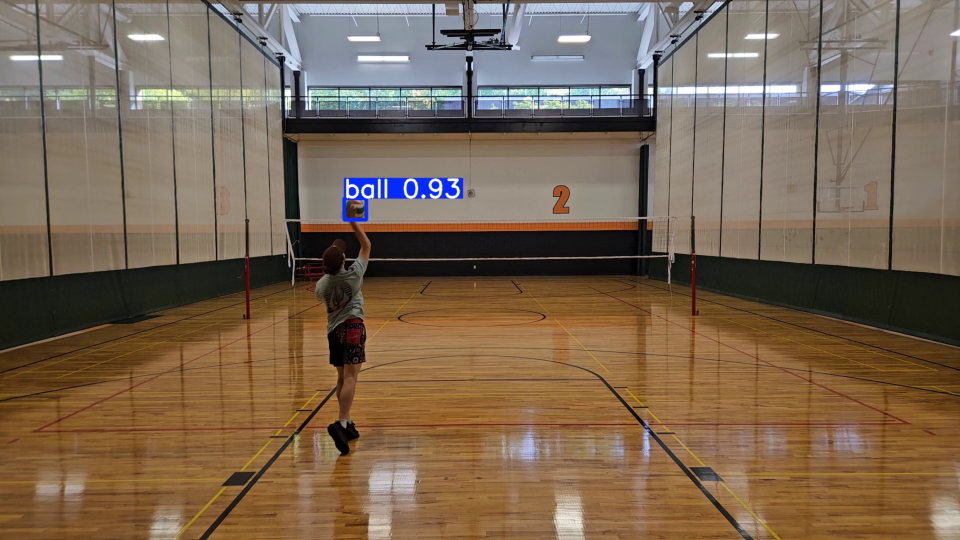
\includegraphics[width=0.8\columnwidth]{assets/sample_detections_serve.pdf}
    }
  
    \subfloat{%
      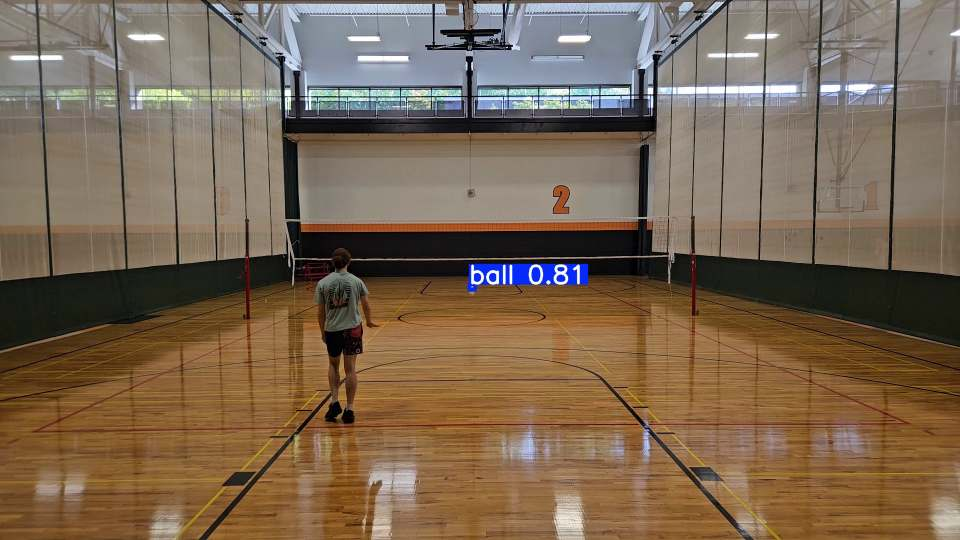
\includegraphics[width=0.8\columnwidth]{assets/sample_detections_landing.pdf}
    }

    \caption{Example YOLOv8 detections on 1080p frames. The ball is often small, blurred, or partially occluded.~(a) Ball detection on serve, (b) Ball detection on landing}
    \label{fig:yolo-detect}
  \end{figure}

Figure~\ref{fig:yolo-detect} shows sample detections on frames with occlusions and blurred, miniscule (less than 10 pixels) balls, illustrating the robustness of the fine-tuned detector.

\subsection{Ball Tracking with SORT and Fragment Merging}

\begin{figure}[!t]
    \centering
    \subfloat{%
      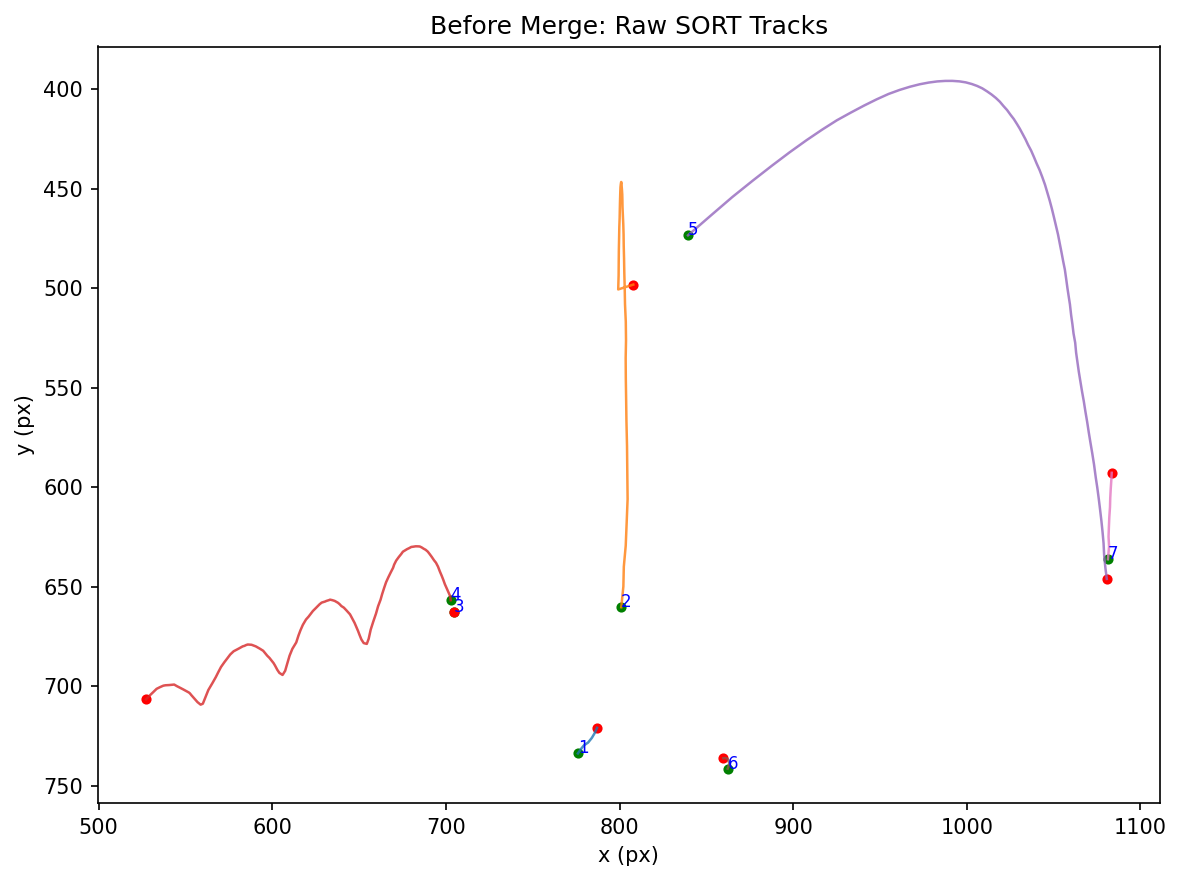
\includegraphics[width=0.9\columnwidth]{assets/sort_merge_before.pdf}
    }
  
    \subfloat{%
      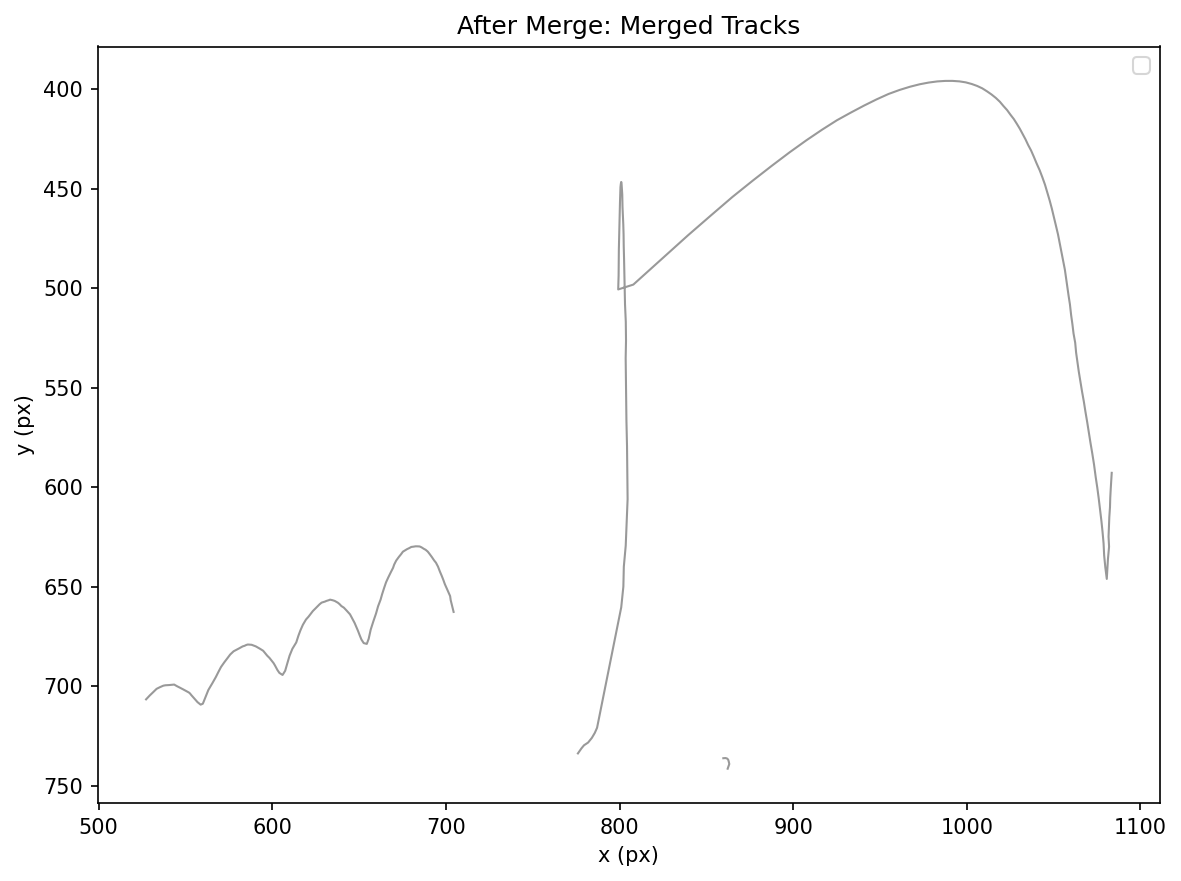
\includegraphics[width=0.9\columnwidth]{assets/sort_merge_after.pdf}
    }
  
    \subfloat{%
      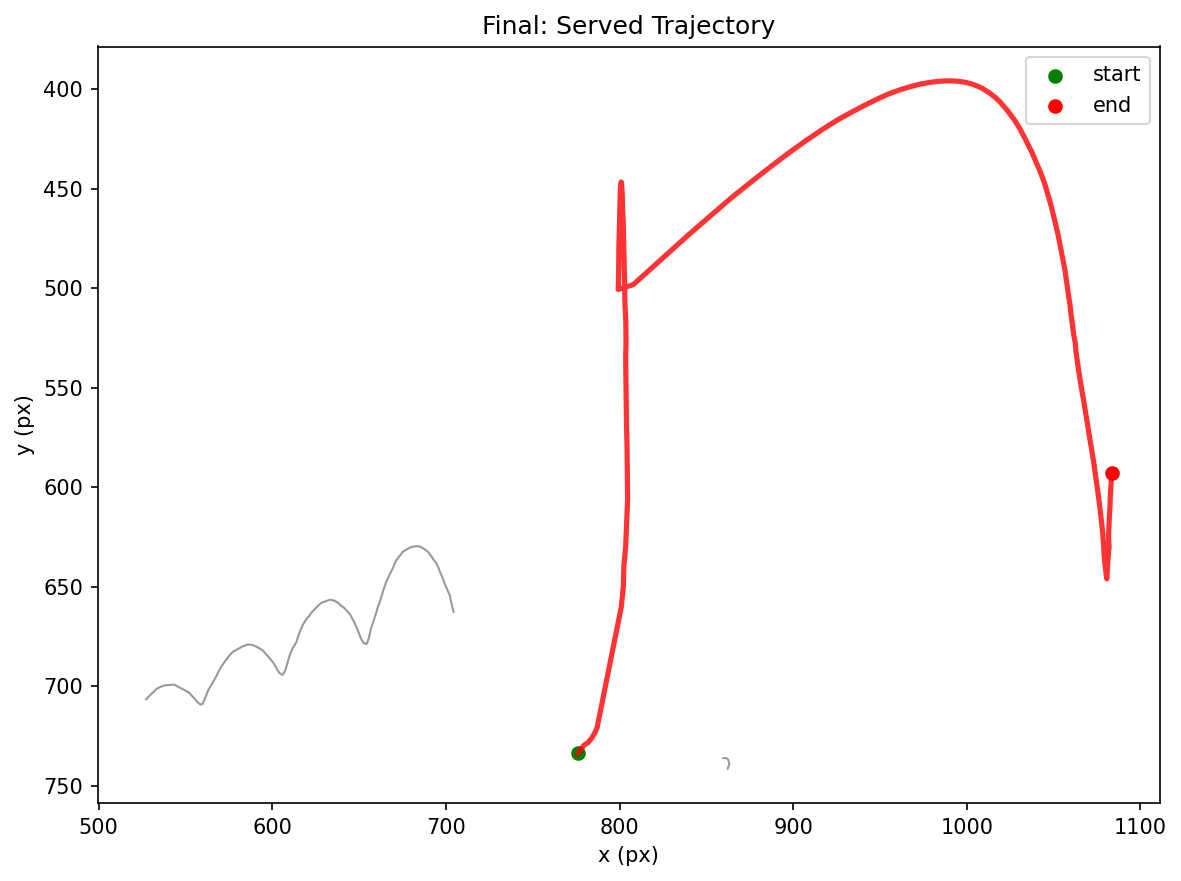
\includegraphics[width=0.9\columnwidth]{assets/sort_merge_final.pdf}
    }
  
    \caption{Trajectory reconstruction stages from detection to final serve path.\\ (a) Raw SORT fragments, (b) Merged trajectories, (c) Selected serve trajectory}
    \label{fig:sort-merge}
  \end{figure}

Although YOLOv8 provides accurate per-frame detections, temporal linking is necessary to form coherent ball trajectories. We use the SORT tracker, which applies a Kalman filter to predict object motion and uses IOU-based Hungarian assignment for frame-to-frame consistency. SORT is well-suited for this task: it is fast, has no re-identification component (unnecessary for a single-object scene), and naturally handles moderate motion blur.

SORT is configured with \texttt{max\_age=30} (allowing up to 30 missed detections before terminating a track), \texttt{min\_hits=1}, and \texttt{iou\_threshold=0.3}. The output of SORT is typically a set of short, fragmented tracks. These fragments arise primarily from occlusions by the server's arm or torso, failures of the detector during the ball's fastest motion, or abrupt appearance changes as the ball rotates.

To reconstruct a single continuous trajectory, we introduce a greedy fragment-merging procedure. Two fragments are considered merge candidates if their temporal gap falls within $[-\mathrm{overlap\_back}, +\mathrm{frame\_gap}]$ and the Euclidean distance between the earlier fragment’s endpoint and the later fragment’s start point is below a spatial threshold. A cost function combining temporal gap and spatial distance ranks merge candidates. Edges are accepted greedily while enforcing a one-incoming, one-outgoing constraint for each fragment and preventing cycles.

Among the merged trajectories, the final serve path is selected using a simple speed-based heuristic that favors longer, faster trajectories. It also ensures the average size of the ball decays through the track, preventing a rolling ball becoming the selected track. Figure~\ref{fig:sort-merge} visualizes the three stages of this process: raw SORT fragments, merged sequences, and the final selected trajectory.

\subsection{Court Calibration via Homography}

To convert image-space trajectories into physical court coordinates, each recording session is calibrated using a planar homography. Unlike methods that require court-line segmentation or multi-camera geometry, our approach uses a simple manual annotation step: the user clicks six distinctive court points visible in the frame using an interactive tool. These points include the four court corners and the two center-line intersections. Their corresponding world coordinates are defined using standard volleyball dimensions, with the origin at the near-left baseline corner, the $x$-axis spanning the nine-meter width, and the $y$-axis extending the full eighteen-meter court length, as shown in Figure~\ref{fig:court_corners}.

Given the image–world correspondences, a $3\times3$ homography matrix $H$ is computed and stored for all serves in that session. Applying $H$ transforms any pixel coordinate $(u,v)$ into metric coordinates $(x,y)$, enabling realistic trajectory overlays, landing-zone assignment, and metric consistency across sessions.

\begin{figure}[!t]
    \centering
    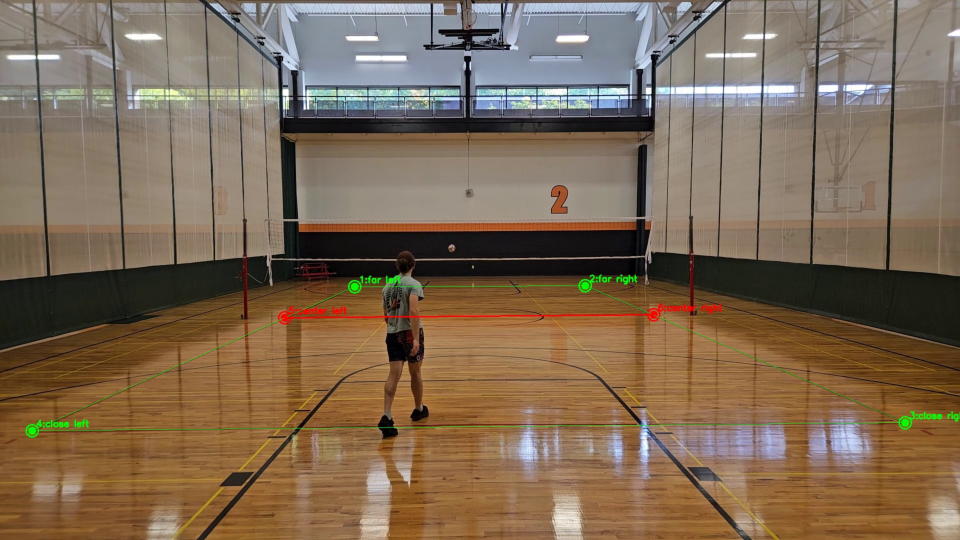
\includegraphics[width=0.8\columnwidth]{assets/court_corners.pdf}
    \caption{Manual annotation of six court reference points allows pixel-to-meter calibration via homography.}
    \label{fig:court_corners}
\end{figure}

\subsection{Trajectory Smoothing}

The selected trajectory consists of per-frame measurements of the ball’s center coordinates and apparent size (computed as $\sqrt{w h}$). These sequences contain noise from detection jitter, bounding-box variation, and tracking uncertainty. To obtain smooth and differentiable signals, we apply a Savitzky–Golay filter~\cite{savitzky1964smoothing} with an adaptive odd window length up to 9 and polynomial order~2. This produces smoothed horizontal and vertical positions, $x_s(t)$ and $y_s(t)$, and smoothed apparent size $s(t)$.

The derivative of vertical position, $dy/dt$, is computed using a finite-difference approximation. This signal is particularly important for landing detection, as a shift from downward to upward velocity after a hit often indicates ground contact and rebound.

\subsection{Hit and Landing Analysis}

The final stage of the pipeline identifies two critical temporal events: the \emph{hit frame}, corresponding to the player's contact with the ball, and the \emph{landing frame}, corresponding to the ball’s first contact with the ground. Both are inferred from the smoothed trajectory signals and their derivatives.

\subsubsection{Hit Detection}

Hit detection uses a hybrid motion–appearance heuristic. Frames before index~20 are ignored to remove early toss noise. The algorithm then identifies a ``near-server'' region where the apparent size exceeds 90\% of its maximum; in this region the ball is physically closer to the camera, encompassing both the toss apex and the hit moment.

Within this region, the toss apex is the minimum of $y_s(t)$ and apparent size. After the apex, the algorithm searches for the earliest window in which apparent size decreases consistently and significantly, indicating that the ball has been struck and is accelerating away from the camera.

This approach is robust to partial occlusions and brief detection dropout, since size changes often persist even when positional noise is present.

\subsubsection{Landing Detection}

Landing detection is performed within a temporal window following the estimated hit frame. Candidate landing frames are identified primarily using the vertical position signal, where the first prominent local maximum in $y(t)$ corresponds to ground contact and rebound. To reduce false positives caused by mid-flight noise or tracking instability, candidates are additionally constrained by apparent ball size: only frames where the smoothed size is below a fixed fraction (0.5) of the maximum observed size are considered valid. This ensures that landing detection occurs only when the ball is sufficiently far from the camera, consistent with floor contact on the far side of the court. As observed in Figure~\ref{fig:landing_analysis} the system combines the use of $y_s(t)$, $dy/dt$, and apparent size in making these calculations.

If no valid vertical-position peak satisfies this size constraint, a fallback strategy is used based on a rolling minimum of the apparent ball size. The candidate frame is refined by selecting the local frame with the largest vertical position while maintaining the size constraint. A final sanity check enforces that the landing frame occurs strictly after the hit frame, preventing degenerate estimates in truncated or failed tracks.

\begin{figure}[!t]
    \centering
    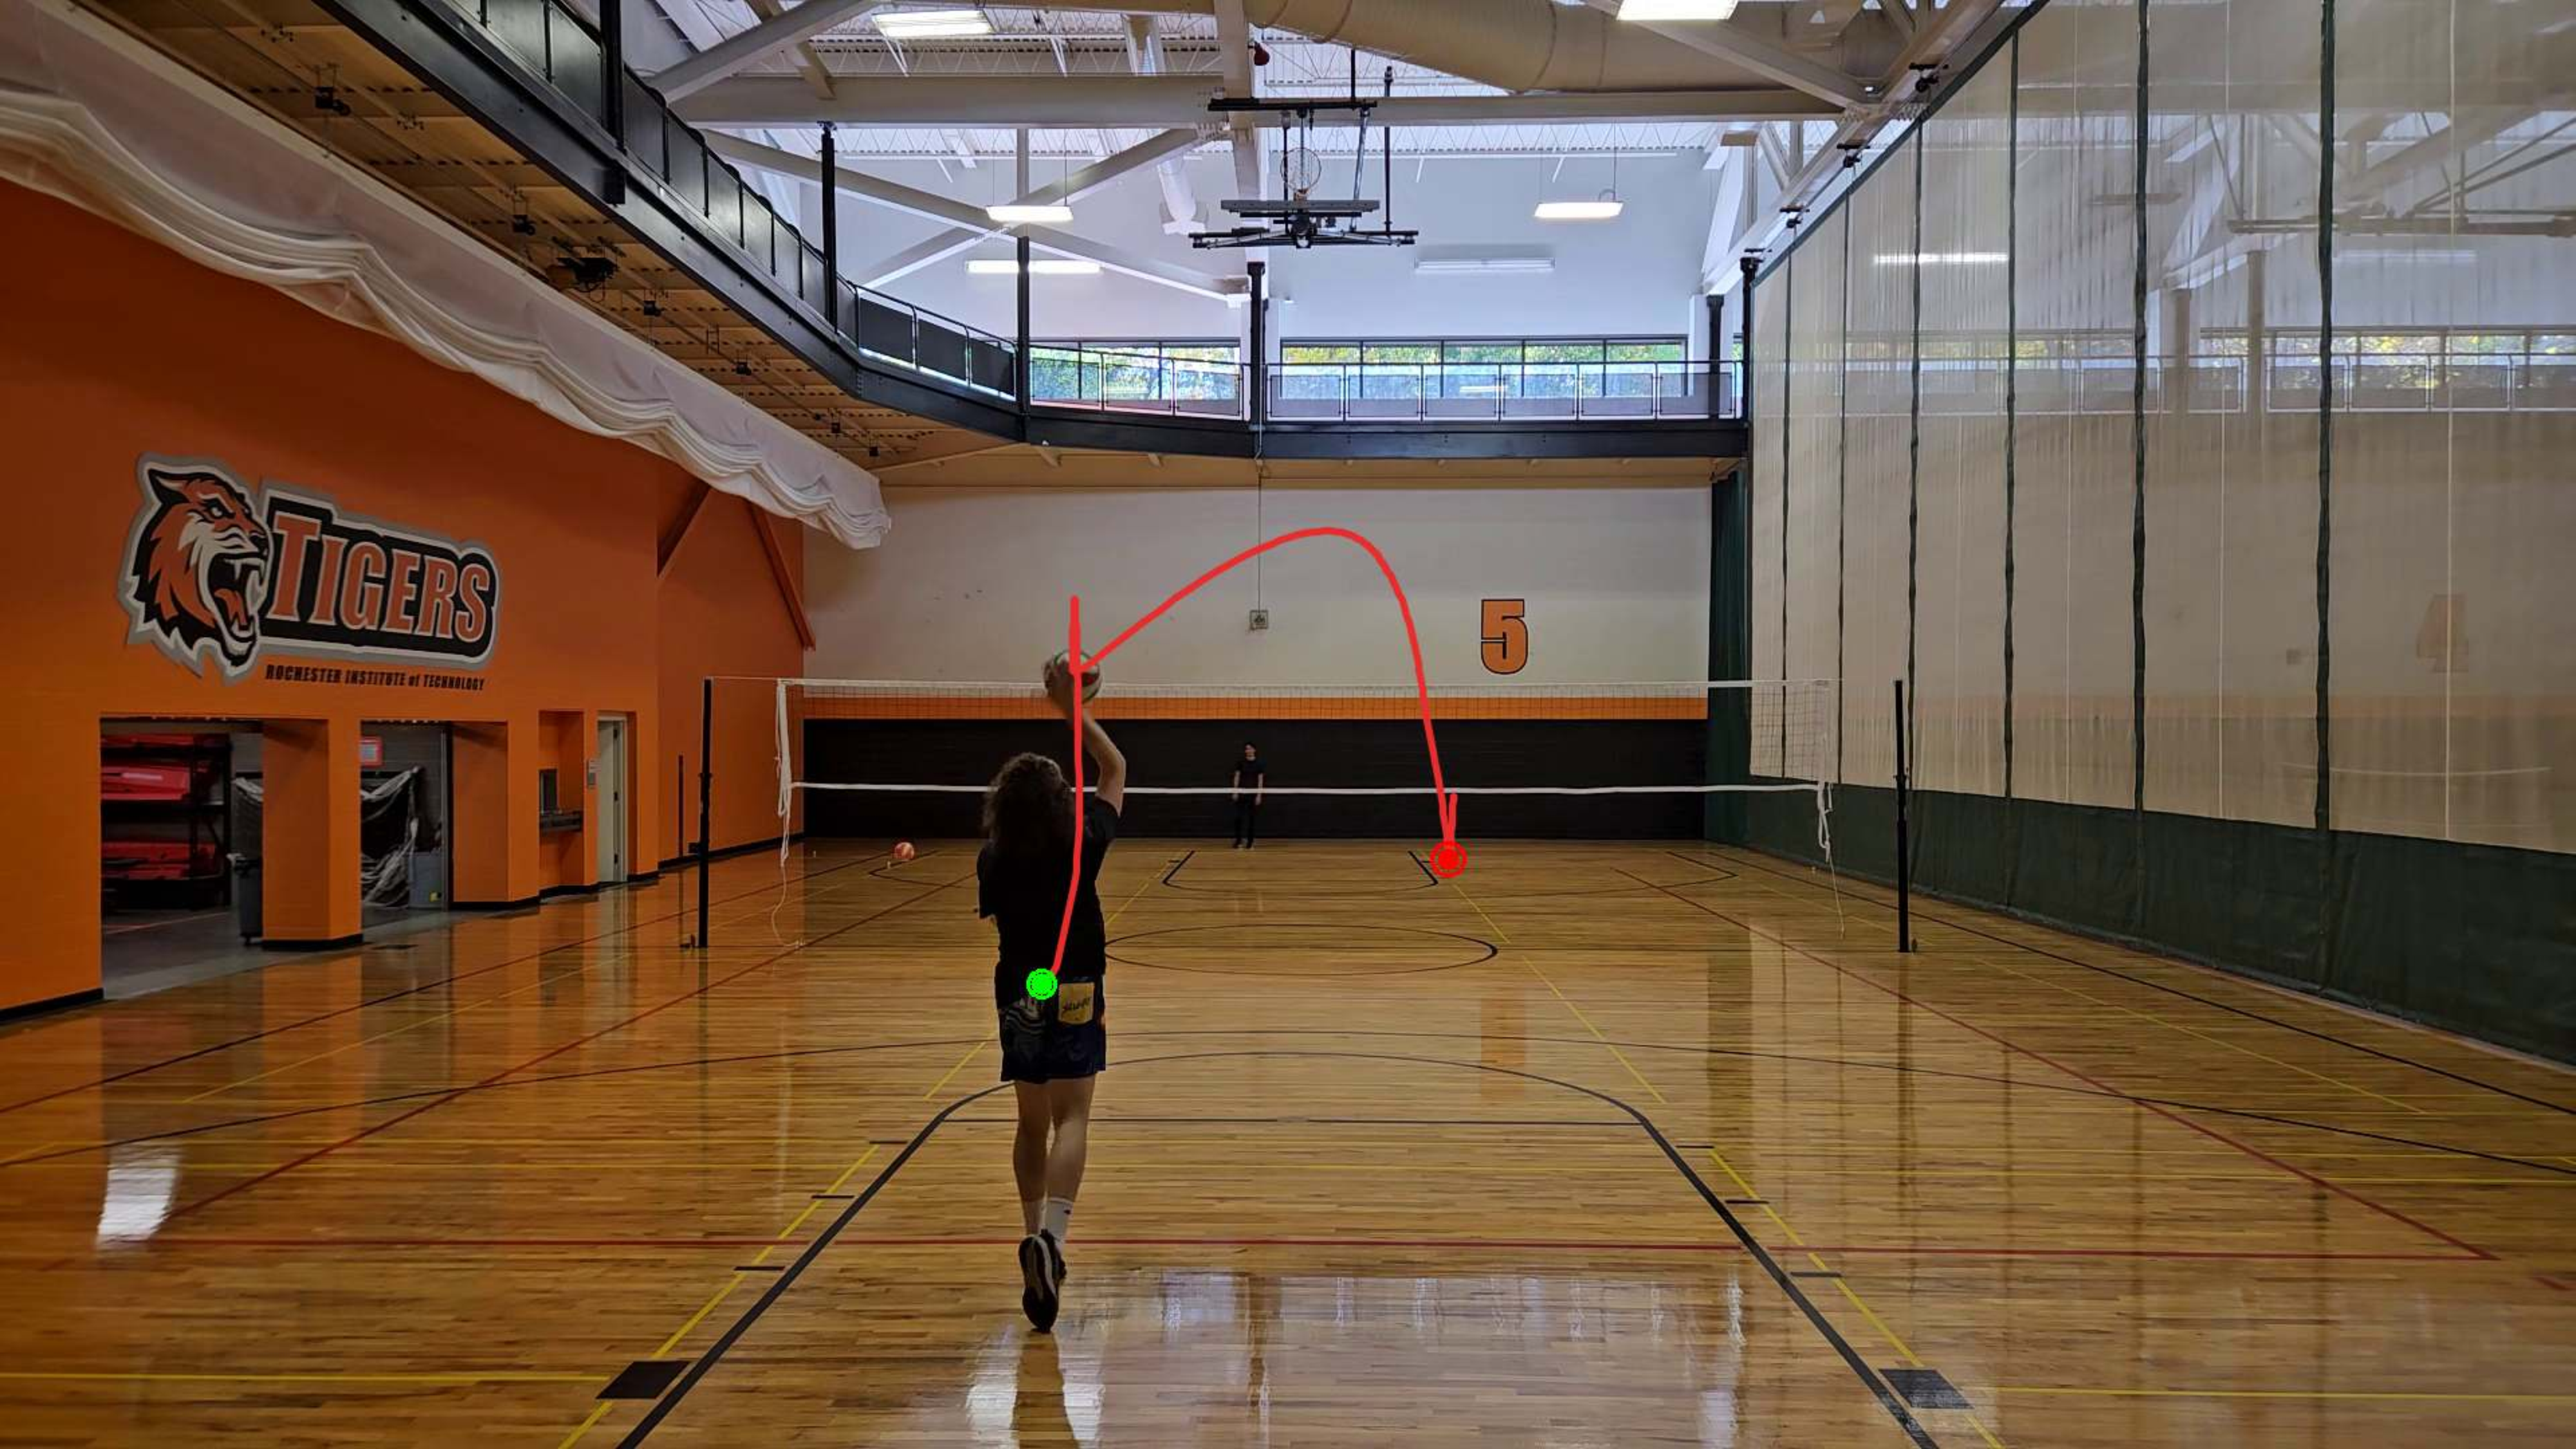
\includegraphics[width=0.8\columnwidth]{assets/trajectory.pdf}
    \caption{Example ball trajectory projected to real-world coordinates using session-specific homography.}
    \label{fig:trajectory}
\end{figure}

\begin{figure}[!t]
    \centering
    \subfloat{%
      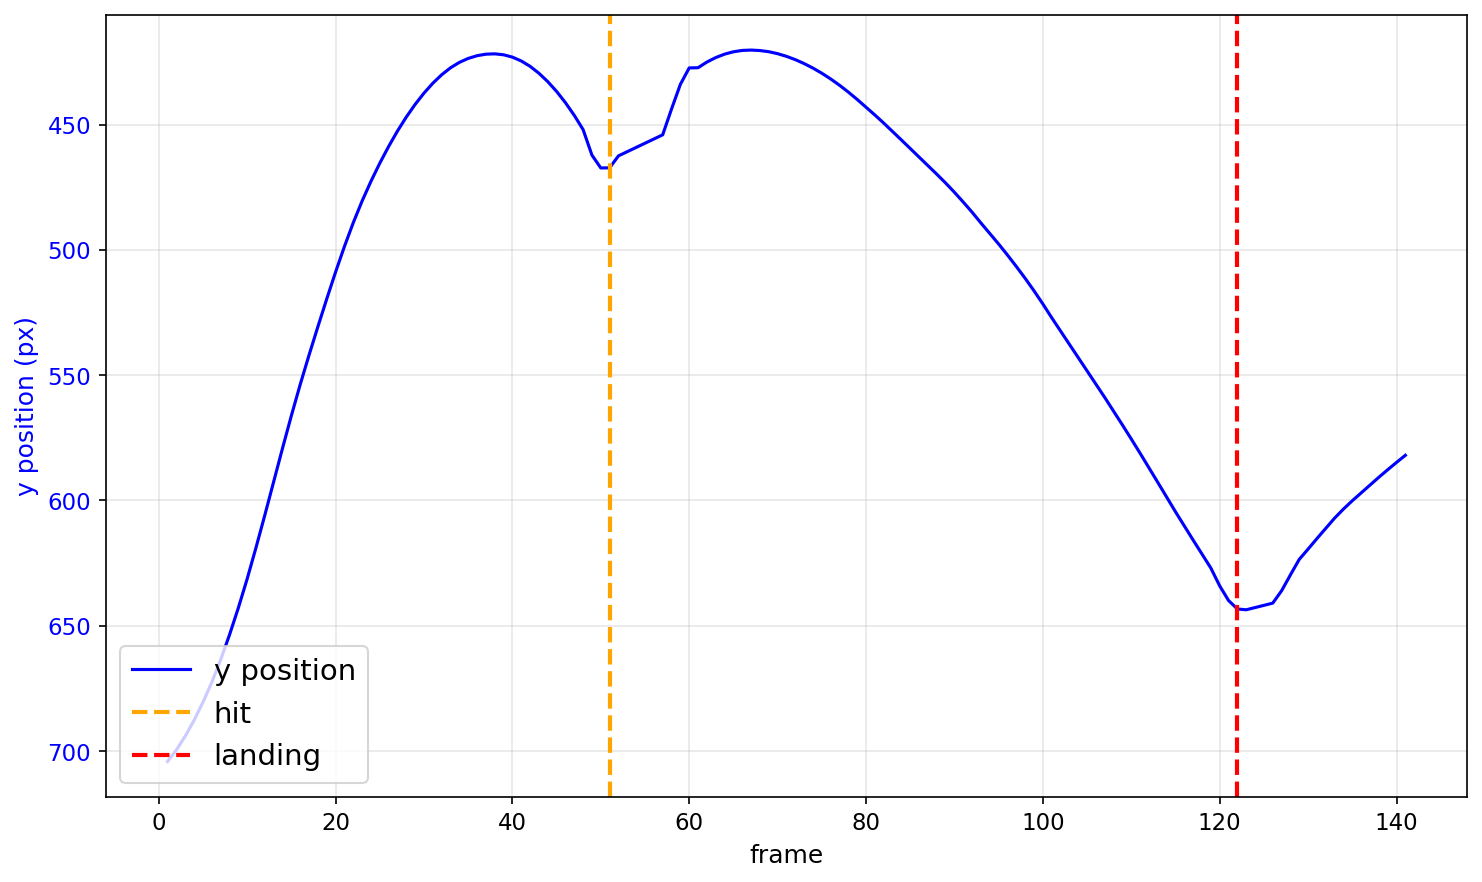
\includegraphics[width=0.9\columnwidth]{assets/landing_analysis_y.pdf}
    }
  
    \subfloat{%
      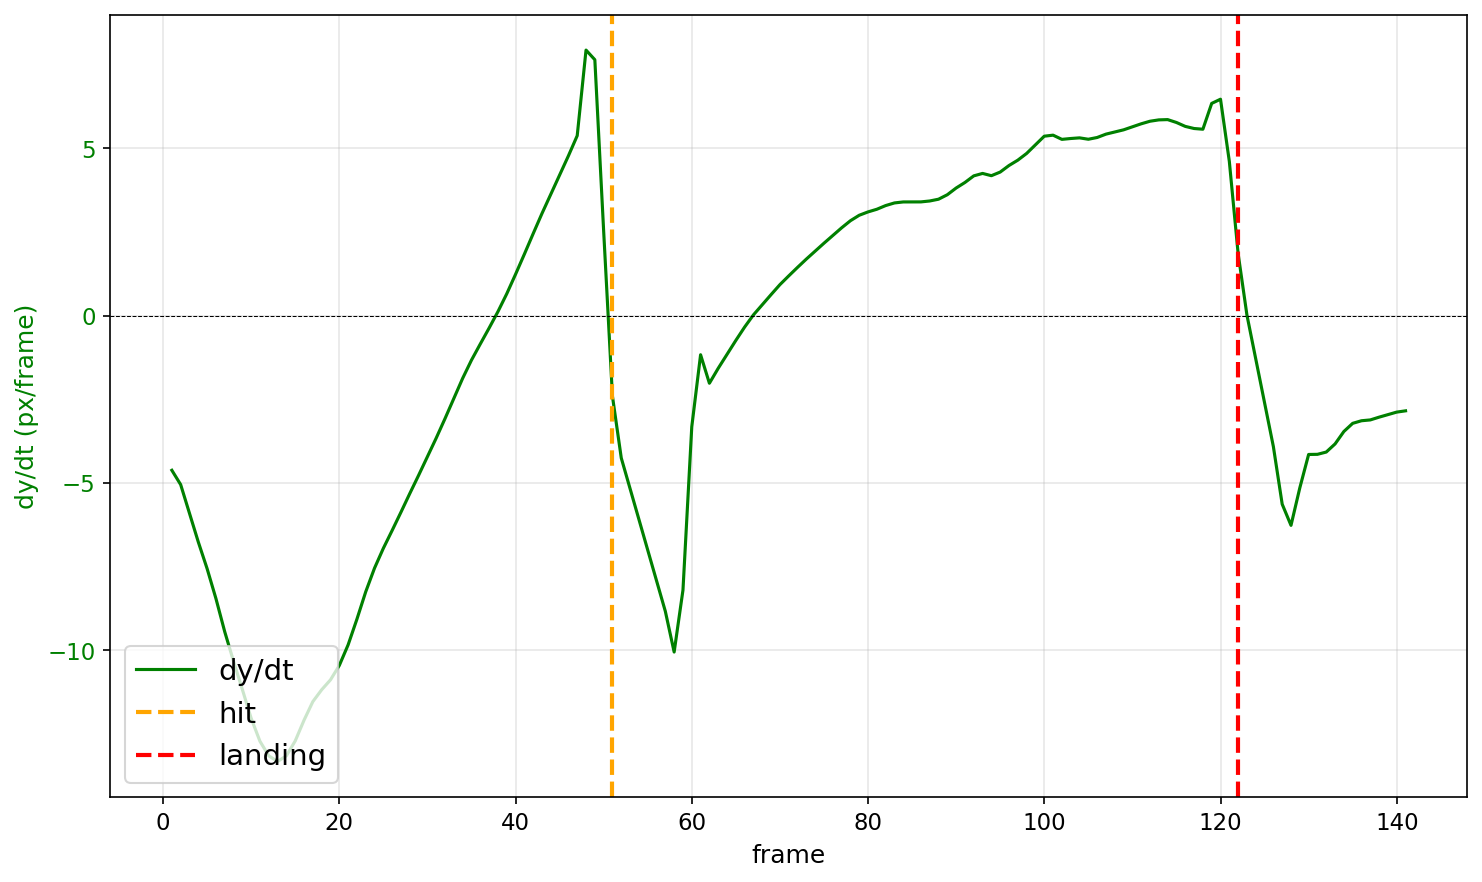
\includegraphics[width=0.9\columnwidth]{assets/landing_analysis_dy.pdf}
    }
  
    \subfloat{%
      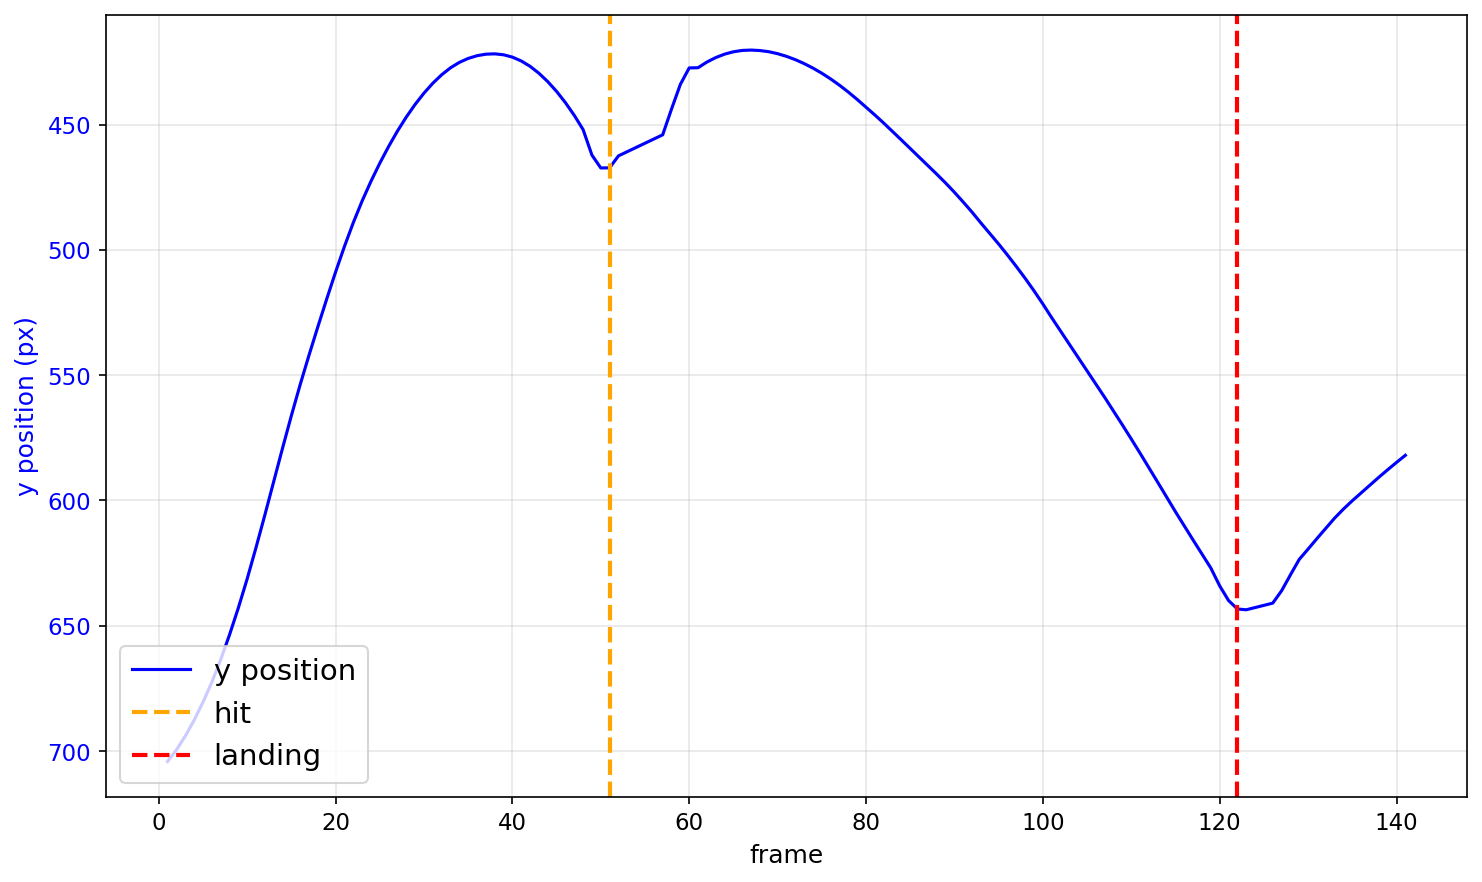
\includegraphics[width=0.9\columnwidth]{assets/landing_analysis_size.pdf}
    }
  
    \caption{Smoothed vertical position, derivative, and apparent size signals used to detect hit and landing events.~(a) Vertical position, (b) Derivative, (c) Apparent size}
    \label{fig:landing_analysis}
  \end{figure}

\subsection{Visualization and Zone Analysis}

Once hit and landing frames are identified, the landing pixel coordinate is projected through the session’s homography to obtain metric $(x,y)$ coordinates on the far side of the court. These coordinates enable serve-level analytics, including trajectory plots (Figure~\ref{fig:trajectory}), landing-point scatter maps, density heatmaps, and accuracy evaluation within FIVB-style zones. All visualizations are produced automatically as part of the user workflow.

The combination of detection, tracking, calibration, and temporal analysis yields a fully automated system capable of extracting quantitative serve characteristics from a single baseline camera.

